\documentclass[reprint, aps, prx, amsmath, amssymb, longbibliography, superscriptaddress]{revtex4-2}

%% don't need amsmath because it is loaded in \documentclass
%% \usepackage{amsmath,amssymb}
\usepackage{graphicx}
\usepackage{epsfig}
\usepackage{mathrsfs,esint}
\usepackage{physics}
\usepackage{relsize}
\usepackage{bbold}
%% \usepackage{float} %% revtex4-2 has a conflict with float
\usepackage{dsfont}
\usepackage{comment}
\usepackage{svg}

%% packages for combining several images into a single figure
%%\usepackage{caption}
%%\usepackage{subcaption}
\usepackage[caption=false]{subfig}

%% Hyperref loaded the last because some packages may redefine \label
\usepackage[bookmarks=true,
   colorlinks=true,
   linkcolor=blue,
   urlcolor=blue,
   citecolor=blue,
   bookmarks=true,
   hyperindex=true
]{hyperref}
%\usepackage{natbib}

% todo package
\usepackage{todonotes}

\definecolor{mediumtealblue}{rgb}{0.0, 0.33, 0.71}
\newcommand{\jk}[1]{{\color{mediumtealblue}#1}}
\newcommand{\al}[1]{{\color{purple}#1}}
\newcommand{\dl}[1]{{\color{red}#1}}


\DeclareMathOperator{\Zn}{\mathbb{Z}_n}
\DeclareMathOperator{\Zthree}{\mathbb{Z}_3}
\DeclareMathOperator{\Ztwo}{\mathbb{Z}_2}
\DeclareMathOperator{\Id}{Id}
\DeclareMathOperator{\diag}{diag}
\DeclareMathOperator{\sgn}{sign}


\begin{document}

\title{From \texorpdfstring{$\Zthree$}{Z3} Rabi model to Potts model}

\author{Anatoliy I. Lotkov}
\affiliation{Department of Physics, University of Basel, Klingelbergstrasse 81, CH-4056 Basel, Switzerland}

\author{Valerii K. Kozin}
\affiliation{Department of Physics, University of Basel, Klingelbergstrasse 81, CH-4056 Basel, Switzerland}


\author{Denis V. Kurlov}
\affiliation{Department of Physics, University of Basel, Klingelbergstrasse 81, CH-4056 Basel, Switzerland}


\author{Jelena Klinovaja}
\affiliation{Department of Physics, University of Basel, Klingelbergstrasse 81, CH-4056 Basel, Switzerland}

\author{Daniel Loss}
\affiliation{Department of Physics, University of Basel, Klingelbergstrasse 81, CH-4056 Basel, Switzerland}

%%%%%%%%%%%%%%


\begin{abstract}
We study the $\Zthree$-symmetric Rabi models in this paper. In particular, we consider 1-mode and 2-mode variants of the $\Zthree$ Rabi model and determine their spectra. Next, we derive a mapping of the 2-mode $\Zthree$ Rabi model onto a qubit-boson ring. This mapping allows us to formulate a possible implementation of the $\Zthree$ Rabi model based on superconducting qubits and provides a context for the previously proposed optomechanical implementation. Furthermore, we propose a physical implementation of the $\Zthree$ Potts model via a chain of $\Zthree$ Rabi models coupled through nearest-neighbor interactions. Finally, we investigate the effects of the disorder on these systems.
\end{abstract}

\maketitle


\section{Introduction}

Quantum simulation has entered a mature phase in which a variety of hardware platforms can reproduce many-body Hamiltonians that are analytically intractable. Trapped-ion chains now implement long-range Ising and lattice-gauge dynamics with tens of qubits \cite{tan_domainwall_2021, kyprianidis_observation_2021,brydges_probing_2019,zhang_observation_2017,martinez_realtime_2016,meth_simulating_2025}; neutral-atom Rydberg arrays routinely emulate spin models on two-dimensional lattices \cite{madjarov_highfidelity_2020,semeghini_probing_2021,scholl_quantum_2021,manovitz_quantum_2025,bernien_probing_2017}; and semiconductor spin-qubit have begun to realize Fermi–Hubbard and other models at the few-plaquette level \cite{dehollain_nagaoka_2020, hensgens_quantum_2017, kiczynski_engineering_2022, vandiepen_quantum_2021, wang_experimental_2022, wang_probing_2023}. These successes show that controlled, programmable devices can already access symmetry breaking, topological order and non-equilibrium critical phenomena that lie well beyond classical reach. A natural next goal is to push such studies toward larger discrete symmetries ($\Zthree$, $\mathbb{Z}_4$, …) and to explore whether the associated phase transitions remain continuous or become first order.

Recent advances in circuit quantum electrodynamics (cQED) provide a complementary route to this goal, focusing on light–matter systems where photons mediate interactions between superconducting qubits\cite{kurpiers_deterministic_2018,vanloo_photonmediated_2013,astafiev_resonance_2010}. In cQED, the quantum Rabi model \cite{braumuller_analog_2017, braak_integrability_2011,hwang_quantum_2015, chen_shortcuts_2021} --- describing a two-level atom coupled to a boson mode --- serves as the canonical building block and possesses a discrete $\Ztwo $ (parity) symmetry. At ultrastrong coupling, chains of Rabi units effectively realize an Ising chain\cite{hwang_largescale_2013}: photon-induced interactions generate nearly degenerate “cat” ground states with macroscopic qubit–cavity entanglement. This connection between discrete symmetry and entangled phases raises a compelling question: what new phenomena emerge when the Rabi symmetry is extended from $\Ztwo$ to $\Zthree$ \cite{albert_quantum_2012, zhang_z_n_2014, sedov_chiral_2020,kozin_quantum_2024}? A threefold generalization links naturally to the paradigmatic three-state Potts model and promises richer symmetry-breaking behavior.

The theoretical appeal of a $\Zthree$ quantum Rabi model is reinforced by growing experimental feasibility. Albert’s generalization of the Rabi Hamiltonian to an $N$-state atom \cite{albert_quantum_2012}established the formal framework. Afterwards, the first implementation of the $\Zthree$ Rabi model based on the optomechanical system was proposed \cite{sedov_chiral_2020}. Now, recent circuit proposals have shown how Josephson-junction networks can implement the $\Zthree$ Potts model using tunable inductive elements \cite{wauters_engineering_2024}. However, a plethora of open questions still remains. Whether a $\Zthree$-symmetric superradiant transition in cQED can be continuous remains unclear. Prior studies of $\Zthree$ analogues of the Dicke model --- for example in chiral waveguide optomechanics --- found predominantly first-order transitions with threefold-degenerate cat states. Here we introduce a tunable model that connects the $\Zthree$ Rabi with the $\Zthree$ Potts model. By varying a coupling parameter, the system evolves from an integrable few-level regime into one that spontaneously breaks the threefold rotational symmetry. 

The rest of the paper is organized as follows. In Sec.~\ref{sec:z3-rabi}, we give a short overview of the $\Zthree$ Rabi model, derive the mapping of the $\Zthree$ Rabi model onto the qubit-boson ring, and illustrate the aforementioned mapping by superconducting-qubit and optomechanical implementations. In Sec.~\ref{sec:potts-model}, we show how the $\Zthree$ Potts model can be simulated by a chain of the $\Zthree$ models and once again illustrate this by superconducting and optomechanical implementations. In the end of Sec.~\ref{sec:potts-model}, we mention the chiral $\Zthree$ Potts model and possibility of its implementation based on a chain of the $\Zthree$ Rabi models. In Sec.~\ref{sec:conclusion}, we conclude. Some additional details are deferred to Apps.~\ref{app:arbitrary-interaction-summary}-\ref{app:disorder}.



\section{\texorpdfstring{$\Zthree$}{Z\_3} Rabi model.}
\label{sec:z3-rabi}

\subsection{Theoretical description}
\label{sec:rabi-theory}

The cental theme of this paper is the $\Zthree$-symmetric Rabi and Potts model as well as the connection between them. In this section, we give a brief description of the $\Zthree$ Rabi model. For the more detailed discussion, we refer the reader to our companion paper \cite{lotkov_cat_}. In particular, we talk about the two-mode variation of the $\Zthree$ Rabi model because it maps onto the qubit-boson ring (see Sec.~\ref{sec:physical-implementation}). It describes the $\Zthree$-symmetric interaction of two boson modes and a qutrit.\todo{explain what qutrit is?} The model's Hamiltonian is
\begin{equation}
\label{eq:2-mode-z3-Rabi}
\begin{aligned}
     H_{\text{R}} = &\Omega_{\text{R}} (\hat a_1^{\dagger} \hat a_1 + \hat a_2^{\dagger} \hat a_2) + B (e^{i\phi} Z + e^{-i\phi} Z^{\dagger}) \\
    &- \lambda (\hat a_1 + \hat a_2^{\dagger}) X - \lambda (\hat a_1^{\dagger} + \hat a_2) X^{\dagger},
\end{aligned}
\end{equation}
where $\hat a_i^{\dagger}\  (\hat a_i)$ with $i = 1,2$ are boson creation (annihilation) operators \footnote{Note that we use hats to distinguish the boson operators, $\hat a,\, \hat a^{\dagger},\, \hat x, \,\hat p$.}, $X$ and $Z$ are $3\times 3 $ matrices generalizing the Pauli matrices (usually referred to as the shift and clock matrices, respectively). The parameters in Eq.~\eqref{eq:2-mode-z3-Rabi} have the following physical meaning: $\Omega_{\text{R}}$ is the frequency of the two boson mode, $B$ and $\phi$ define the qutrit energy levels, and $\lambda$ is the coupling strength between the boson modes and the qutrit.

The $\Zthree$ shift $X$ and clock $Z$ matrices are a standard tool for describing the qutrit systems. \todo{cite?} They are defined by
\begin{equation}
\label{eq:shift-clock-matreces}
    X = \begin{pmatrix} 
         0 & 0 & 1 \\
         1 & 0 & 0 \\
         0 & 1 & 0 
        \end{pmatrix}, \quad
    Z = \begin{pmatrix}
         1 & 0 & 0 \\
         0 & \omega & 0 \\
         0 & 0 & \omega^2
        \end{pmatrix},
      \end{equation}
where $\omega = \exp[2\pi i/3]$ is the principle cubic root of unity. The clock and shift matrices are unitary, $ X X^{\dagger} = \mathbb{1}, \, Z Z^{\dagger} = \mathbb{1}$, but not hermitian, $ X^{\dagger} \neq X, \, Z^{\dagger} \neq Z$. Therefore, the analogy between them and the Pauli matrices is not full. But the $X$ and $Z$ matrices allow us to generalize the qubit Pauli group $\mathcal{P}_2 = \langle \pm i^j \omega_z^k \omega_x^l\rangle_{j,k,l = 0}^1$ to the qutrit Pauli group $\mathcal{P}_3 = \langle \pm \omega^j Z^k X^l\rangle_{j,k,l= 0}^{2}$ \todo{cite?}. The elements of the group $\mathcal{P}_3$ generate a basis for the qutrit operators.

The $\Zthree$ symmetry group for the qutrit appears naturally as a part of the qutrit Pauli group $\mathcal{P}_3$. Actually, there are two $\Zthree$ subgroups in the $\mathcal{P}_3$ group: generated by the powers of the matrix $X$ and $Z$. While both subgroups are conjugate to each other, here we choose the subgroup generated by the $Z$ matrix, $\Zthree = \langle Z^k \rangle_{k=0}^2$. The boson part of the $\Zthree$ symmetry is simply a residue of the bosonic $\mathrm{U(1)}$ symmetry. As a result, the $\Zthree$ symmetry generator has the following form:
\begin{equation}
     R_{\text{R}} = \exp\left[\frac{2\pi i}{3}(a_1^{\dagger}  a_1 -  a_2^{\dagger}  a_2)\right] Z.
\end{equation}
As a consequence of the symmetry, the number of the first boson excitations minus the number of the second boson excitations and plus the number of the qutrit excitations is conserved modulo 3. While this requirement is not particularly straightforward, it is necessary for the rest of our arguments to work. For the details, we refer to the companion paper \cite{lotkov_cat_}.

One of the key ingridients in our $\Zthree$ Potts model is the strong boson-qutrit interaction. In particular, we are interested in what is usually called the deep-strong coupling regime in the Rabi model literature, $\lambda \gtrsim \Omega_R$. Also, we require the low magnetic field limit, $ B \ll \Omega_R$. This coupling regime leads to the full entanglement between the boson and qutrit degrees of freedom. Specifically, the three lowest eigenstates turn out to be the $\Zthree$ cat states \cite{lotkov_cat_} that allows us to implement the $\Zthree$-symmetric nearest neighbour interaction required for the Potts model,
\begin{equation}
\label{eq:three-cat-states}
    |\psi_k\rangle = \frac{1}{\sqrt{3}}\sum\limits_{l=0}^2 \omega^{lk}|\omega^{-l} \lambda/\Omega_{\text{R}}\rangle_{\hat a_1}|\omega^l \lambda/\Omega_{\text{R}}\rangle_{\hat a_2} |\omega^{-l} \rangle,
\end{equation}
where $\hat a_1$ ($\hat a_2$) subscripts denote that it is a coherent state of the first (second) boson mode.  The $\ket{\psi_k}$ states are the $\Zthree$ generalization of the ordinary cat states $\ket{+\alpha} \pm \ket{-\alpha}$. As you see, the ordinary ($\Ztwo$) cat states are a linear combination of two coherent states with parameters $\pm\alpha$. In the $\Zthree$ case, $|\psi_k\rangle$ states are a linear combination of three coherent states with parameters $\omega^i \alpha, \, i = 0,1,2$ instead. Also, for the two-mode $\Zthree$ Rabi model $\ket{\psi_k}$ is a joint cat state of the two boson modes and a qutrit. In case of the $\Zthree$ Rabi model, the coherent parameter is expressed through the model's coupling constants, $\alpha = \lambda/\Omega_R$. Having reviewed the necessary information of the $\Zthree$ Rabi model, we can move on to the model's mapping onto the qubit-boson ring.

\subsection{Qubit--boson ring}
\label{sec:physical-implementation}

In this section, we show how the two-mode $\Zthree$ Rabi model~\eqref{eq:2-mode-z3-Rabi} emerges
in the single-qutrit-excitation sector of a three-site qubit-boson (QB) ring with a
nearest-neighbor coupling. This is the central construction of this paper. It allows us to propose a superconducting circuit implementation of the $\Zthree$ Rabi model below. Also, the optomechanical implementation for the $\Zthree$ Rabi model is based on a similar construction \cite{sedov_chiral_2020}.  Here, we work with a homogeneous chain with the periodic boundary condition. In App.~\ref{app:arbitrary-interaction-summary}, a similar argument is walked through for a chain with an arbitrary connectivity. The QB ring Hamiltonian is
\begin{equation}
\label{eq:physical-hamiltonian}
  \begin{aligned}
    H_{\text{QB}} &= \epsilon \sum_{j=0}^{2} \sigma_j^z
      + \Omega_{\text{QB}} \sum_{j=0}^{2} \hat b_j^{\dagger} \hat b_j
      + V_{\text{QB}},
      \\
    V_{\text{QB}} &= g \sum_{j=0}^{2}
      \bigl( \sigma_j^{+} \sigma_{j+1}^{-}
      e^{ i ( \hat x_j - \hat x_{j+1} ) } + \text{h.c.} \bigr),
  \end{aligned}
\end{equation}
where $\sigma_j^z$ correspond to the qubit degrees of freedom, while $\hat b_j^{\dagger}$ ($\hat b_j$) is the creation (annihilation) operator of the $j$th boson. Next, $\epsilon$ defines the Zeeman splitting of the qubit energy levels; $g$ is the coupling strength; $\Omega_{\text{QB}}$ is the boson frequency with $m_{\text{QB}}$ \todo{Mention that mass is necessary as an additional parameter} being the mass of the corresponding harmonic oscillator. Consequently, we define coordinate and momentum operators for each boson mode as
\begin{align}
    \hat x_j &= \sqrt{\frac{1}{2 m_{\text{QB}} \Omega_{\text{QB}}}}\left(\hat b_j + \hat b_j^{\dagger}\right) \\
    \hat p_j &= \sqrt{\frac{m_{\text{QB}} \Omega_{\text{QB}}}{2 }}\left(\hat b_j - \hat b_j^{\dagger}\right).
\end{align}
\begin{comment}

\begin{equation}
  \hat a_j = \sqrt{\frac{m_{\text{QB}} \Omega_{\text{QB}}}{2}}\, \hat x_j
           + i \sqrt{ \frac{1}{2 m_{\text{QB}} \Omega_{\text{QB}}} }\, \hat p_j.
\end{equation}
\end{comment}

The system has a $\mathrm{U(1)}$ symmetry conserving the total z axis spin projection\todo{Check how it is named in aps journals} $\hat S^z = \sum_j
\sigma_j^z$, because it commutes with the Hamiltonian~\eqref{eq:physical-hamiltonian}, $[ \hat H_{\text{QB}}, \hat S^z ] = 0$. Consequently, we consider not the full Hilbert space but only a certain sector with a specific total z axis spin projection, i.e., 
the single-excitation sector
\begin{equation}
\label{eq:single-excitation-sector}
  \mathcal H_{\text{QB},1} = \operatorname{Span}\bigl\{ |
    \uparrow\downarrow\downarrow\rangle,
    |\downarrow\uparrow\downarrow\rangle,
    |\downarrow\downarrow\uparrow\rangle \bigr\}.
\end{equation}

To prove that the QB ring~\eqref{eq:physical-hamiltonian} restricted to the single excitation sector $\mathcal{H}_{\text{QB,1}}$~\eqref{eq:single-excitation-sector} is equivalent to the $\Zthree$ Rabi model, we first apply several algebraic transformations to the Hamiltonian $H_{\text{QB}}$~\eqref{eq:physical-hamiltonian}. To start with, we use the spin-dependent momentum translation to simplify the interaction term $V_{\text{QB}}$~\eqref{eq:physical-hamiltonian}. Then, we apply the Fourier transform, it decouples one of the boson modes from the rest of the system. Afterwards, the resulting Hamiltonian is restricted to the single-excitation sector $\mathcal{H}_{\text{QB},1}$~\eqref{eq:single-excitation-sector}. We obtain the two-mode $\Zthree$ Rabi model, which is brought to the canonical form with some final adjustments.

\paragraph{Spin-dependent momentum translation.}
Applying the unitary operator
$S = \prod_j e^{ i \sigma_j^z \hat x_j / 2 }$ removes the exponentials in
$\hat V_{\text{QB}}$ and yields
\begin{align}
\label{eq:after-momentum-translation}
    S^{-1} \hat H_{\text{QB}} S &= \epsilon \sum_{j} \sigma_j^z
      + \Omega_{\text{QB}} \sum_j \hat b_j^{\dagger} \hat b_j
      + \frac{1}{2 m_{\text{QB}}} \sum_j \hat p_j \sigma_j^z \notag
      \\
      &\quad + \frac{3}{4 m_{\text{QB}}}
      + g \sum_{j}
        \bigl( \sigma_j^{+} \sigma_{j+1}^{-} + \sigma_j^{-} \sigma_{j+1}^{+} \bigr).
\end{align}

The qubit interaction is now purely spin-spin, at the price of an additional
spin-boson term proportional to $\hat p_j \sigma_j^z$.

\paragraph{Fourier transform.}
Introducing momentum-space operators $\hat b(k)$ and spin operators $S^{\pm}(k)$ via the Fourier transform, $\hat b(k)= \tfrac{1}{\sqrt{3}}\sum_{j}e^{-2\pi i jk/3}\hat b_j$, $ S^z(k)= \tfrac{1}{\sqrt{3}}\sum_{j}e^{-2\pi i jk/3}\sigma_j^z$ (and analogously for the spin raising $S^+$ and lowering $S^-$operators), we
bring Eq.~\eqref{eq:after-momentum-translation} to
\begin{equation}
\label{eq:after-fourier}
  \begin{aligned}
    &\hat H_{\text{FT}} = \epsilon \sum_{k=0}^{2} S^{z}(k)
      + \Omega_{\text{QB}} \sum_{k=0}^{2} \hat b^{\dagger}(k) \hat b(k)
                         + \frac{3}{4 m_{\text{QB}}} \\
     &+\frac{1}{2 m_{\text{QB}}} \sum_{k=0}^{2} \hat p(k) S^{z}(-k)
            + g \sum_{k=0}^{2} \bigl( S^{+}(k) S^{-}(-k) + \text{h.c.} \bigr),
  \end{aligned}
\end{equation}
where The zero-momentum ($k=0$) boson mode
couples to the $S^z(k=0)$, which is conserved. Hence, it actually decouples from the rest system. We are left with only two boson modes that are required for the $\Zthree$ Rabi model.

\paragraph{Restriction to $\mathcal H_{\text{QB},1}$.}
To restrict the Hamiltonian~\eqref{eq:after-fourier} to the single-excitation sector $\mathcal{H}_{\text{QB},1}$~\eqref{eq:single-excitation-sector}, we identify the single-excitatioin spin states with qutrit states, $\ket{0} \equiv \ket{\uparrow\downarrow\downarrow}$, $ \ket{1} \equiv \ket{\downarrow\uparrow\downarrow}$, and $ \ket{2} \equiv \ket{\downarrow\downarrow\uparrow} $. After discarding constants and the decoupled mode, we obtain
\begin{equation}
  \begin{aligned}
    &\hat H_{\text{QB},1} = \Omega_{\text{QB}} \sum_{k=1}^{2} \hat b^{\dagger}(k)
      \hat b(k) + g \bigl( X + X^{\dagger} \bigr)
      \\
      &+ i \sqrt{ \frac{\Omega_{\text{QB}}}{6 m_{\text{QB}}} }
        \Bigl[ -( \hat b(1) - \hat b^{\dagger}(2) ) Z
        - ( \hat b(2) - \hat b^{\dagger}(1) ) Z^{\dagger} \Bigr],
  \end{aligned}
\end{equation}
where $X$ and $Z$ matrix act on the qutrit formed by the single-excitation sector $\mathcal{H}_{\text{QB},1}$~\eqref{eq:single-excitation-sector}.

\paragraph{Final rearrangement.}
The Hadamard transform on the spin degrees of freedom, combined with a global
bosonic $\mathrm{U(1)}$ phase rotation, brings the Hamiltonian to the canonical
$\Zthree$ two-mode Rabi form,

\begin{align}
\label{eq:effective-rabi}
    &\hat H_{\text{R}} = \Omega_{\text{QB}}
      \bigl( \hat a^{\dagger}_1 \hat a_1 + \hat a^{\dagger}_2 \hat a_2 \bigr)
      + g \bigl( Z + Z^{\dagger} \bigr) \notag
      \\
      &- \sqrt{ \frac{\Omega_{\text{QB}}}{6 m_{\text{QB}}} }
      \Bigl[ ( \hat a_1 + \hat a^{\dagger}_2 ) X
        + ( \hat a_2 + \hat a^{\dagger}_1 ) X^{\dagger} \Bigr],
\end{align}
where we identified $\hat a_k \equiv \hat b(k)$ and $\hat a_k^{\dagger} \equiv \hat b^{\dagger}(k)$ for $k = 1,2$. The identification with Eq.~(\ref{eq:2-mode-z3-Rabi}) leads to
\begin{equation}
\label{eq:QB-RM-parameter-mapping}
  \Omega_R = \Omega_{\text{QB}},
  \quad B = g,
  \quad \phi = 0,
  \quad \lambda = \sqrt{ \frac{\Omega_{\text{QB}}}{6 m_{\text{QB}}} }.
\end{equation}

For the sake of completeness, we provide the ``magnetic'' term explicitly,
\begin{equation}
\label{eq:superconducting-magnetic-term}
  g \bigl( Z + Z^{\dagger} \bigr) =
  \begin{pmatrix}
    2 g & 0 & 0 \\
    0 & -g & 0 \\
    0 & 0 & -g
  \end{pmatrix}.
\end{equation}

As shown, the single-excitation sector $\mathcal{H}_{\text{QB},1}$ of the QB ring~\eqref{eq:physical-hamiltonian} indeed simulates the $\Zthree$ Rabi model~\eqref{eq:2-mode-z3-Rabi}. Moreover, the mapping is exact. We emphasize superconducting qubits as a natural platform for engineering the
interaction~\eqref{eq:physical-hamiltonian}, although analogous constructions are
possible in, for example, optomechanical settings \cite{sedov_chiral_2020}.


\subsubsection{Why so complicated?}

The implementation of the $\Zthree$ Rabi model proposed in the previous section is considerably more complicated than the usual $\Ztwo$ Rabi model ones. To obtain the $\Ztwo$ Rabi model it is enough to simply couple a qubit with a boson in a naive way. Therefore, one may wonder if these complications are necessary. However, the straightforward generalization of the $\Ztwo$ Rabi model to higher Rabi models does not work due to fundamental obstacles. It turns out to be considerably more difficult to get a $\Zthree$ symmetric interaction. In this section, we try to explain why.

There are two most common ways to get a two-level quantum system. It is possible to use a spin as a two-level system  \cite{bosco_fully_2022,felicetti_quantum_2017,skogvoll_tunable_2021} or two levels in anharmonic oscillator, e.g., the Rabi model describes a superconducting qubit coupled to a cavity in the ultra-strong coupling regime \cite{niemczyk_circuit_2010,forn-diaz_ultrastrong_2017,yoshihara_superconducting_2017,vlasiuk_cavityinduced_2023, kozin_quantum_2024,chen_singlephotondriven_2017,ricco_reshaping_2022}. Therefore, to get a $\Ztwo$ Rabi model, one has to take either a spin or an anharmonic oscillator and couple it to a boson mode using $\hat V = \sigma_x \hat x_{\text{boson}}$.

Both ways are easily generalized to the $\Zthree$ case. To get a spin-based three-level system we just have to take spin $1$ system. However, in this case, we obtain an interaction through the spin-1 representation of $s^x$ instead of $X$.
\begin{equation}
    s^x= \begin{pmatrix} 0 & \sqrt{2} & 0 \\ \sqrt{2} & 0 & \sqrt{2} \\ 0 & \sqrt{2} & 0 \end{pmatrix}
\end{equation}
It is easy to see that it is not $\Zthree$-symmetric. Hence, the spin $1/2$ representation of the $SU(2)$ group is a convenient special case that, unfortunately, does not generalize. It does not prove that it is impossible to build a $\Zthree$ symmetric system out of spins as we have shown, or higher $\Zn$ symmetric systems \cite{hutter_parafermions_2015} in general. But it still shows why we require rather complicated ways to achieve it.

The second way to obtain a $\mathbb{Z}_2$ Rabi model is to use two levels of an anharmonic oscillator. Consequently, in the $\mathbb{Z}_2$ case $\sigma^x$ operator is a restriction of the coordinate operator of the anharmonic oscillator $ \hat x_{\text{an}} = (\hat b_{\text{an}} + \hat b_{\text{an}}^{\dagger})/\sqrt{2} $ to the two lowest levels. On the contrast, if we restrict it to 3-level system, we get
\begin{equation}
    \hat x_{\text{an}} = \frac{1}{\sqrt{2}}\begin{pmatrix} 0 & \sqrt{1} & 0 \\ \sqrt{1} & 0 & \sqrt{2} \\ 0 & \sqrt{2} & 0 \end{pmatrix}
\end{equation}
As a result, the $\Ztwo$ Rabi model based on the anharmonic oscillator does not generalize to the higher $\Zn$ Rabi models as well.

These obstacles make an experimental $\Zn$‑Rabi realization non‑trivial, motivating our proposal. The rationale provided in this section is in no way a formal proof. However, the argument should serve as an intuition as to why the $\Zthree$ Rabi is less straightforward to engineer than its more well-known analogue. The model we proposed in the previous section solves this problem by having an inherent $\Zthree$ symmetry. It originates from the translational symmetry of a ring.

\subsection{Superconducting circuit implementation}
\label{sec:superconducting-implementation}

In this section, we discuss how to implement the QB ring Hamiltonian~\eqref{eq:physical-hamiltonian} in a superconducting-qubit system. The obvious choice for boson modes is a cavity (modeled by an LC circuit for our purposes). For the qubit ($\sigma_i$)  we consider superconducting charge qubits \cite{bouchiat_quantum_1998,nakamura_coherent_1999,lehnert_measurement_2003,makhlin_quantumstate_2001}, because we want the qubit eigenstate to be a charge state. An extensive discussion on the charge qubits we use is provided in App. \ref{app:charge-qubit}. Here, we only want to comment that the qubit eigenstates are $|0\rangle, |1\rangle$ defined by $\hat n |0\rangle = 0, \, \hat n |1\rangle = |1\rangle$, where $\hat n$ is the capacitor charge operator. Below, to denote a linear span of these states we use $\mathcal{V}_k = \operatorname{Span}\{|0\rangle_k, \, |1\rangle_k\}$, where $k$ is the number of the qubit.

Fig.~\ref{fig:superconducting-Rabi} shows a superconducting realization of the three‑site QB ring, discussed in Sec.~\ref{sec:physical-implementation}. Each horizontal (as shown in Fig.~\ref{fig:superconducting-Rabi}) branch of the circuit corresponds to site $i = 0,1,2$ of the qubit-boson ring. The $i$th boson $\mathrm{B}i$ and qubit $\mathrm{Q}i$ are implemented by the LC circuit and SC qubit on the $i$th branch respectively. The JJs on on the vertical (once again as shown in Fig.~\ref{fig:superconducting-Rabi}) segments of the circuit on the right of Fig.~\ref{fig:superconducting-Rabi} are responsible for the interaction term in $H_{QB}$~\eqref{eq:physical-hamiltonian} \cite{siewert_aspects_2000,rasmussen_controllable_2019,shafranjuk_twoqubit_2006,allman_tunable_2014,hu_controllable_2007}. On Fig.~\ref{fig:superconducting-Rabi}, the characteristic parameters of every circuit element are also shown: LC circuit's conductor and inductor have capacitance $C_{\text{B}}$ and inductance $L_{\text{B}}$ respectively. The qubit's JJ and capacitance have critical current $I_{\text{Q}}$ and capacitance $C_{\text{Q}}$ respectively. The coupling JJs on the right have critical current $I_{\text{R}}$. For clarity, we omit any elements that are necessary for an actual experimental implementation, e.g., read‑out resonators, flux‑bias lines, and filtering components.

\begin{figure}[t]
  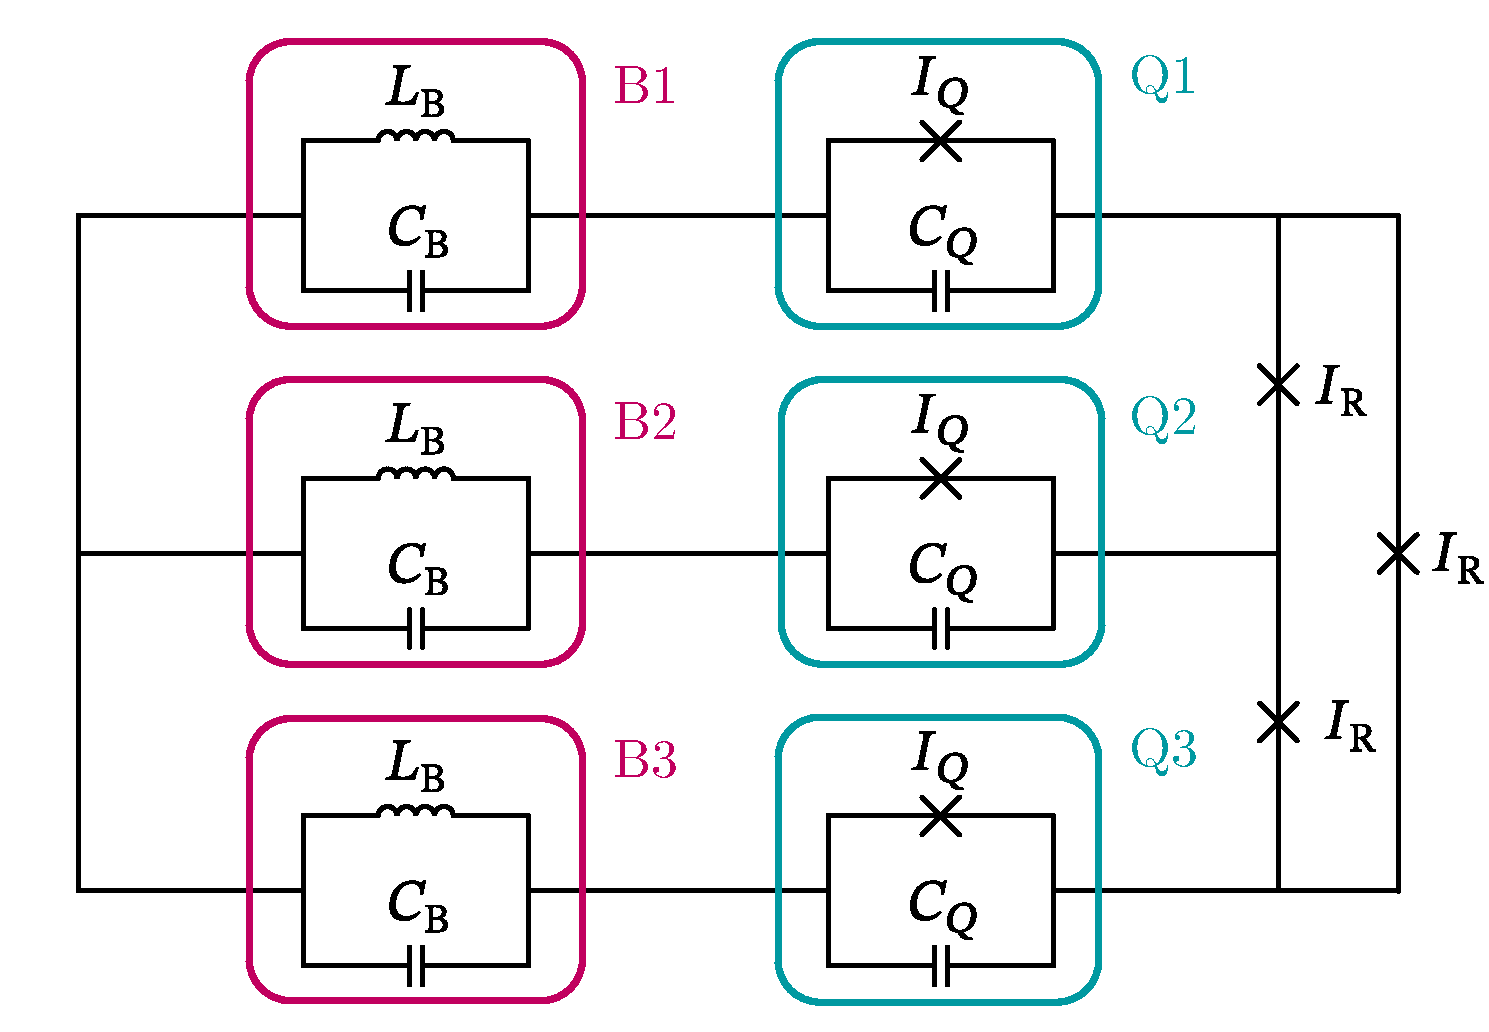
\includegraphics[width=\linewidth]{pics/SC_Rabi_circuit_with_contours.pdf}
  \caption{Superconducting circuit implementation of the 2-mode $\Zthree$ Rabi model $\hat H_{\text{R}}$. The LC circuits $(L_{\text{B}}, C_{\text{B}})$ host the boson modes B1, B2, and B3 (marked by the magenta color); the charge qubits $(I_{\text{Q}}, C_{\text{Q}})$ correspond to the qubit degrees of freedom Q1, Q2, and Q3 (marked by the cyan color); Josephson junctions $I_{\text{Rabi}}$ are responsible for the interaction term in the qubit-boson ring. Altogether, the circuit is described by the Hamiltonian~\eqref{eq:physical-hamiltonian}.}
  \label{fig:superconducting-Rabi}
\end{figure}

Next, we argue why this circuit models the Hamiltonian~\eqref{eq:physical-hamiltonian}. Without the coupling JJs, the LC circuits and qubits do not interact with each other and are described by a free Hamiltonian:
\begin{equation}
    H = \sum_{i = 0}^2  H_{LC, i}(\hat \phi_i, \hat q_i) + \sum_{i = 0}^2 H_{Q,i}(\hat \varphi_i, \hat n_i),
\end{equation}
where $ \hat\phi_i, \hat q_i$ are the magnetic flux and the capacitor charge of the $i$th LC circuit, while $\hat \varphi_i, \hat n_i$ are the JJ superconducting phase and capacitor charge of the qubit. The LC circuit Hamiltonian is obviously $ H_{LC, i} = q_i^2/(2C) + \phi_i^2/(2L)$. Meanwhile, we leave the qubit Hamiltonian $\hat H_{Q,i} $ generic to allow different qubit types. However, we require the qubit to be a charge qubit and satisfy the following properties:
\begin{align}
   H_{Q}\bigg|_{\mathcal{V}} = \begin{pmatrix} \bra{0_i} H_Q\ket{0_i} & \bra{0_i} H_Q \ket{1_i} \\ \bra{1_i} H_Q \ket{0_i} & \bra{1_i} H_Q \ket{1_i} \end{pmatrix} = \epsilon \sigma_z,
\end{align}
where the qubit states $\ket{0_i},\ket{1_i}$ are the charge operator eigenstates $ \hat q_i \ket{0_i} = Q \ket{1_i}, \, \hat q_{i} \ket{1}_i = (Q+1)\ket{1}_i$ with $ Q \in \mathbb{Z}$. $\mathcal{V}_i = \operatorname{Span}\{\ket{0_i},\, \ket{1_i}\}$ is a qubit Hilbert space, i.e, a computational subspace of the full Hilbert space of the qubit system $ \hat H_{Q,i}$. Due to this property, the operator $ e^{i\hat \varphi_i} $ acts on the qubit subspace $\mathcal{V}_i$ as a raising operator:
\begin{equation}
  \begin{aligned}
    &e^{i\hat\varphi_i}\bigg|_{\mathcal{V}_i} = \begin{pmatrix} \bra{0_i} e^{i\hat\varphi_i} \ket{0_i} & \bra{0_i} e^{i\hat\varphi_i} \ket{1_i} \\ \bra{1_i} e^{i\hat\varphi_i} \ket{0_i} & \bra{1_i} e^{i\hat\varphi_i} \ket{1_i} \end{pmatrix} = \sigma^+,
  \end{aligned}
\end{equation}
because $[e^{i\hat \varphi}, \hat n] = e^{hat \varphi}$.

If we now connect the $i$th and $(i+1)$th circuit branches with a JJ, it creates a cycle in the circuit. As a result, the fluxes and the superconducting phases have to satisfy a requirement:
\begin{equation}
  \hat \phi_i + \hat\varphi_i + \hat\phi_R - \hat\varphi_{i+1} - \hat\phi_{i+1} = 2\pi N, \, \text{where}\ N \in \mathbb{Z}.
\end{equation}
In other words, the superconducting phase $\hat \phi_R$ of the coupling JJ is not an independent degree of freedom. Therefore, for the corresponding term in the Hamiltonian we obtain:
\begin{equation}
    V_{\text{SC QB},j} = I_{\text{R}} \cos(\hat \phi_R) =  I_{\text{R}}\cos(\hat \phi_j + \hat \varphi_j - \hat \phi_{j+1} - \hat \varphi_{j+1}).
\end{equation}


As we are only interested in qubit states $|0\rangle_k,\, |1\rangle_k$, we restrict the JJ term $\hat V_{\text{SC QB},j}$ to the qubit Hilbert subspace $\mathcal{V}_j\otimes \mathcal{V}_{j+1}$:
\begin{equation}
\begin{aligned}
    &V_{\text{SC QB},j} \bigg |_{\mathcal{V}_j\otimes \mathcal{V}_{j+1}} = \\
    &=\frac{I_{\text{R}}}{2}\left(e^{i(\hat\varphi_j - \hat\varphi_{j+1})} e^{i(\hat\phi_j - \hat\phi_{j+1})} + h.c. \right) \bigg|_{\mathcal{V}_j\otimes \mathcal{V}_{j+1}} \\
    &=\frac{I_{\text{R}}}{2}\left(e^{i(\hat\varphi_j - \hat\varphi_{j+1})} \sigma_j^- \sigma_{j+1}^+ + h.c. \right).
\end{aligned}
\end{equation}
Here we used the fact that $e^{\pm i\hat\phi}$ acts as a raising/lowering operator for the charge qubit: $e^{i\hat\phi}|_{\mathcal{V}} = \sigma^+$. Hence the need for charge qubits rather than flux or phase qubits.

The Josephson junction coupling between two pairs of an LC circuits and a charge qubits gives us precisely the interaction term we wanted. As a result, we conclude that the system depicted in Fig.~\ref{fig:superconducting-Rabi} is described by the Hamiltonian~\eqref{eq:physical-hamiltonian}.  The qubit-boson ring couplings can be expressed by the circuit parameters:
\begin{equation}
\begin{aligned}
    &\epsilon = \frac{\delta}{2 C_Q},\,
    \Omega_{QB} = \left(\sqrt{L_{\text{B}}C_{\text{B}}}\right)^{-1/2}, \\
    &m_{QB} = C_{\text{B}}, \, g = \frac{I_{\text{R}}}{2}.
\end{aligned}
\end{equation}
For details of the $\epsilon$ computation, see App.~\ref{app:charge-qubit}. 

Finally, applying Sec.~\ref{sec:physical-implementation} argument we deduce that the circuit is described by the $\Zthree$ Rabi model. Two practical notes follow from this construction. (i) Replacing each coupling JJ by a dc SQUID makes $g \propto I_{\mathrm{R}}$ tunable (including sign control via flux bias) and allows us to imprint controlled phase offsets around the ring, thereby realizing the ``magnetic'' term with a phase different from Eq.~\eqref{eq:superconducting-magnetic-term}. (ii) The device can be initialized at $g\simeq 0$ with the three qubits and three LC modes effectively decoupled; adiabatic ramp of $g$ then reach the target operating point, while standard dispersive readout on auxiliary resonators provides state discrimination. Taken together, these considerations make the circuit of Fig.~\ref{fig:superconducting-Rabi} a realistic platform for probing $\Zthree$ Rabi model dynamics across coupling regimes without invoking a rotating-wave approximation.


\subsection{Optomechanical implementation}
\label{sec:optomechanical-implementation}

\begin{figure}
    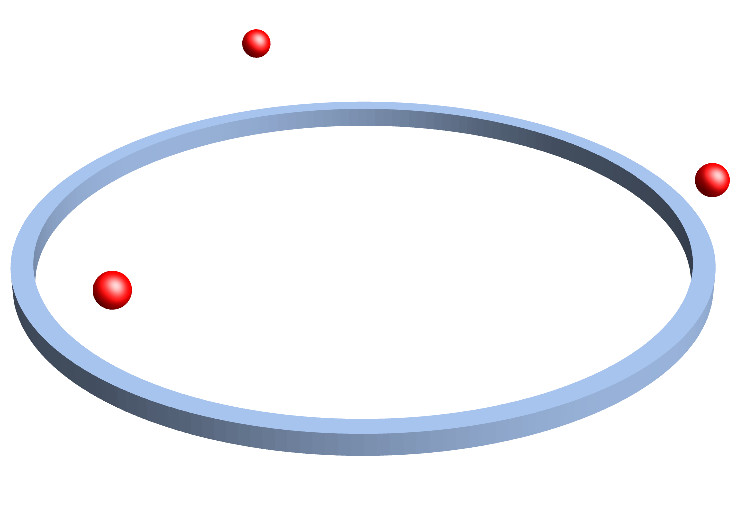
\includegraphics[width=0.8\linewidth]{pics/optomechanical_Rabi_pic.pdf}
    \caption{Schematic illustration of the optomechanical implementation of the 2-mode $\Zthree$ Rabi model $\hat H_{\text{R}'}$ \cite{sedov_chiral_2020} The red spheres are trapped ions carrying two-level systems; their vibrational modes are the bosons from the qubit-boson ring. The blue ring is the chiral waveguide that facilitates the interaction in the qubit-boson ring. The system is described by the Hamiltonian $\hat H_{\text{OM}}$ (\ref{eq:optomechanical-qb-ring}).}
    \label{fig:optomechanical-rabi}
\end{figure}

Another possible physical platform for the $\Zthree$ Rabi model is an optomechanical system consisting of three spins whose vibrational modes are boson degrees of freedom. They are connected by a circular waveguide that acts as an interaction medium between the spins and the vibrational phonons (first proposed in \cite{sedov_chiral_2020}). Although challenging to realize, this platform illustrates the generality of our approach. In this section, we outline how the $\Zthree$ Rabi model arises in this model, for the extended discussion we refer the reader to the original paper \cite{sedov_chiral_2020}. 

The optomechanical model in question is described by the following Hamiltonian:
\begin{equation}
\label{eq:optomechanical-qb-ring}
\begin{aligned}
    \hat{H}_{\text{OM}}&=\sum\limits_{j=0}^2 \zeta_j \hat{c}_j^{\dagger} \hat{c}_j + 
 \epsilon \sum_{j=0}^2 \sigma_j^z + \Omega_{\text{OM}} \sum_{j=0}^2 \hat{b}_j^{\dagger} \hat{b}_j \\
    &+\gamma \sum_{k, j=0}^2 \left[\sigma_j^{+} \hat{c}_k e^{i k\left[R \phi_j+\hat x_j\right]}+\text {h.c.}\right] \text {, }
\end{aligned}   
\end{equation}
where $\hat c_j^\dagger$ ($\hat c_j$) is the waveguide photon creation (annihilation) operator; $\sigma^z_j$,$\sigma_j^+$, and $\sigma_j^-$ is the ion spin degree of freedom; $\hat b^{\dagger}_j$ ($\hat b_j$) are the ion vibrational phonon creation (annihilation) operators with $\hat x_j = (\hat b_j + \hat b_j^{\dagger})/\sqrt{2}$ being the canonical coordinate operator. The parameters are the following: 
$\zeta_k = v k$ is the waveguide photon dispersion, $\epsilon$ is the spin Zeeman splitting, $\Omega_{\text{OM}}$ is the phonon frequency, and $\gamma$ is the coupling strength.

Using the Schrieffer-Wolff transformation \cite{bravyi_schrieffer_2011}, we can integrate out the photons degrees of freedom to get the Hamiltonian in the form we want:
\begin{equation}
\begin{aligned}
&\hat{H}_{\text{OM,eff}}=  \epsilon \sum_j \sigma_j^z + \Omega_{\text{OM}} \sum_j \hat{b}_j^{\dagger} \hat{b}_j \\
& -\frac{\gamma^2}{2v} \sum_{i<j}\left[i \sigma_i^{+} \sigma_j^- e^{i q R \phi_{i j}} e^{i \eta\left(\hat{b}_i+\hat{b}_i^{\dagger}-\hat{b}_j-\hat{b}_j^{\dagger}\right)}+\text {h.c.}\right].
\end{aligned}
\end{equation}
The Hamiltonian is a bit different from~\eqref{eq:physical-hamiltonian}. It is treated in App. \ref{app:arbitrary-interaction-summary} and gives rise to the following $\Zthree$ Rabi model:
\begin{equation}
\begin{aligned}
    &\hat H_{\text{R}'}= - \frac{\gamma^2}{2v} (e^{-5\pi i/6} Z + e^{5\pi i/6} Z^{\dagger}) \\
    &+ \Omega_{\text{OM}} (\hat b_1^{\dagger} \hat b_1 + \hat b_2^{\dagger} \hat b_2) \\
    &- \frac{\Omega_{\text{OM}}^{1/2} \eta}{6^{1/2}}\left[(\hat b_1 + \hat b_2^{\dagger}) X  + (\hat b_2 + \hat b_1^{\dagger}) X^{\dagger}  \right]
\end{aligned}
\end{equation}
which differs from the $\Zthree $ Rabi model we acquired in the superconducting circuit context only by the $\Zthree$ ``magnetic'' term's phase $\varphi = - 5\pi/6$.

We can explicitly write down the ``magnetic'' term
\begin{equation}
    - \frac{\gamma^2}{2v} (e^{-5\pi i/6} Z + e^{5\pi i/6} Z^2) = \begin{pmatrix}
        \frac{\sqrt{3}\gamma^2}{2v} & 0 & 0 \\ 0 & -\frac{\sqrt{3}\gamma^2}{2v} & 0 \\ 0 & 0 & 0 
    \end{pmatrix}.
\end{equation}
As one can see, the non-zero ``magnetic'' term's phase $\varphi$ leads to all the eigenvalues being non-degenerate. Compare it to Eq.~\eqref{eq:superconducting-magnetic-term}.

As a result the optomechanical system~\eqref{eq:optomechanical-qb-ring} provides another way to realize the $\Zthree$ Rabi model~\eqref{eq:2-mode-z3-Rabi}. This implementation uses the waveguide as a mediator for the qubit-boson interaction $V_{\text{QB}}$~\eqref{eq:physical-hamiltonian}, which is a bit more complicated compared to the superconducting implementation (Fig.~\ref{fig:superconducting-Rabi}). Nevertheless, the optomechanical system~\eqref{eq:optomechanical-qb-ring} still models the Rabi model through the mechanism described in Sec.~\ref{sec:physical-implementation}.



\section{\texorpdfstring{$\Zthree$}{Z3} Potts model}
\label{sec:potts-model}

\subsection{Theoretical description}
\label{sec:theoretical-potts}


The $\Zthree$ Potts model \cite{wu_potts_1982} is a one-dimensional chain of three-level systems -- qutrits -- with a global $\Zthree$ symmetry. It  originates from statistical physics as a straightforward generalization of the Ising model  \cite{wu_potts_1982,baxter_critical_1982}. Nowadays, the Potts model often appears in the context of qudit quantum computations \cite{aharonov_polynomial_2007,okada_efficient_2019}. However, the direct experimental realization of the Potts model still does not exist. One of the goals of this paper is to propose such an experimental realization based on $\Zthree$ Rabi models. To achieve this, we generalize the idea of building an Ising model by coupling a chain of $\Ztwo$ Rabi models, proposed by Hwang \cite{hwang_largescale_2013}, to the $\Zthree$-symmetric case.

The $\Zthree$ Potts model Hamiltonian is
\begin{equation}
\begin{aligned}
\label{eq:potts-hamiltonian}
H_{\text{P}} =& f_{\text{P}} \sum\limits_{n=1}^L \left(e^{i\phi}Z_n + e^{-i\phi}Z_n^{\dagger}\right) \\
  &+  J_{\text{P}} \sum\limits_{n=1}^L \left( X_n X_{n+1}^{\dagger} + X_n^{\dagger} X_{n+1}\right),
\end{aligned}
\end{equation}
where $X_n$ and $Z_n$ are the shift and clock matrices~\eqref{eq:shift-clock-matreces} acting on the $n$th qutrit. $f _\text{P}$ describes the strength of a single-site potential, $J_{\text{P}}$ is the coupling strength of $\Zthree$-symmetric nearest-neighbor interaction.

As we have already discussed before, it is difficult to obtain a $\Zthree$ symmetry in an arbitrary three-level system chain. But we have already learned how to construct a $\Zthree$ Rabi model. We use it as a building block for the $\Zthree$ Potts model. We assemble a chain of the $\Zthree$ Rabi models. Then, the three cat-states in the $n$th $\Zthree$ Rabi models~\eqref{eq:three-cat-states} correspond to the three states on the $n$th site of the Potts model $ |j\rangle_n = |\psi_j\rangle_n $ for $j=0,\, 1,\, 2$. In the deep-strong limit of the Rabi model~\eqref{eq:2-mode-z3-Rabi}, $ \lambda \gg \Omega_R$,  the higher energy states are effective decoupled from $|\psi_j\rangle$ states.

The main reason why it is convenient to build the Potts model from the Rabi models is that the boson degrees of freedom in the Rabi model allow us to obtain a $\Zthree$-symmetric interaction. The reasoning is simple: the Rabi model's $\Zthree$ symmetry acting on bosons is a residue of a usual $\mathrm{U(1)}$ boson symmetry. Consequently, if we take a $\mathrm{U(1)}$ symmetric interaction of the boson modes on the neighbor sites in the Rabi model chain, then it is $\Zthree$-symmetric by default. And the simplest $\mathrm{U(1)}$-symmetric boson interaction is just a hopping term $\hat a_n^{\dagger} \hat a_{n+1} + \textrm{h.c.}$ As a result, to obtain the $\Zthree$ Potts model we need to take a chain of $\Zthree$ Rabi models and couple them by the boson hopping term:
\begin{equation}
\label{eq:coupled-rabi}
\begin{aligned}
    &H_{\text{R chain}} = \\
    &\sum\limits_{n=1}^L H_{\text{R}, n} + J \sum\limits_{n=1}^L \sum\limits_{k=1}^2\left( \hat a_{n,k}^{\dagger} \hat a_{n+1,k} + \hat a_{n+1,k}^{\dagger} \hat a_{n,k}\right),
\end{aligned}
\end{equation}
where $n$ is a chain-site subscript and $k$ is a number of the boson mode in the $ \Zthree $ Rabi model. We claim that this Hamiltonian gives us precisely the $\Zthree$ Potts model, when we restrict it to the Hilbert space $\bigotimes_n\mathcal{R}_n$ generated by the three cat states on the sites $n=1,\dots,L$.

Within the Rabi qutrit subspace,  $\hat a_{n,k}$ acts as a permutation between the cat states:
\begin{equation}
    \hat a_{n,k} |\psi_i\rangle_n = (\lambda/\Omega_{\textrm{R}})|\psi_{i+1}\rangle_n. 
\end{equation}
For the creation operator it is a little bit more complicated:
\begin{equation}
\begin{aligned}
    &\hat a_{n,k}^{\dagger} |\psi_i\rangle_n =  (\lambda/\Omega_{\textrm{R}})|\psi_{i-1}\rangle_n + \delta, \,\text{where} \\
    &|\delta|^2 = 1.
\end{aligned}
\end{equation}
In the deep-strong coupling~\cite{kozin_cavityenhanced_2025,kozin_schottky_2025} regime $\lambda/\Omega_{\text{R}} \gg 1$, we can neglect $\delta$. As a result, in the Rabi qutrit subspace the creation/annihilation operators act as cyclic permutations: $\hat a_{n,k}|_{\mathcal{R}} = (\lambda/\Omega_{\textrm{R}}) X$, $\hat a_{n,k}^{\dagger}|_{\mathcal{R}} \approx (\lambda/\Omega_{\textrm{R}}) X^{\dagger}$. Consequently, in this sector the coupled Rabi chain is equivalent to the Potts model:

\begin{equation}
\begin{aligned}
    J &\sum\limits_{k=0}^{2} \left(\hat a_{n,k}^{\dagger} \hat a_{n+1,k} + \hat a_{n+1,k}^{\dagger} \hat a_{n,k}\right) = \\
    &3(\lambda/\Omega_{\textrm{R}})^2 J\left(X_n^{\dagger} X_{n+1} + X_{n+1}^{\dagger} X_n\right).
\end{aligned}
\end{equation}
Therefore, we have $J_{\text{P}} = 3(\lambda/\Omega_{\textrm{R}})^2 J$.
\todo{Add closing remarks.}


\subsubsection{Underlying qubit-boson ring}
\label{sec:underlying-qb-ring}

In the previous section, we showed how to construct the $\Zthree$ Potts model out of a chain of the $\Zthree$ Rabi models. However, each Rabi model is itself implemented by a QB ring [see Sec.~\ref{sec:physical-implementation}]. Here, we show how the underlying QB rings should be coupled to get the boson-hopping interaction~\eqref{eq:coupled-rabi} for the Rabi models. It turns out to be rather straightforward. The hopping term between the QB ring bosons $\hat b_{n,j}$ and $\hat b_{n,j}^{\dagger}$ give us precisely the hopping term between the $\Zthree$ Rabi model bosons $\hat a_{n,k}$ and $\hat a_{n,k}^{\dagger}$ since the Fourier transform does not change the form of the boson hopping interaction:
\begin{equation}
\begin{aligned}
    &\sum\limits_{j=0}^2 \left(\hat b_{n,j}^{\dagger} \hat b_{n+1,j} + \hat b_{n+1,j}^{\dagger} \hat b_{n,j}\right) \\
    &=\sum\limits_{k=0}^{2} \left(\hat b_{n}^{\dagger}(k) \hat b_{n+1}(k) + \hat b_{n+1}^{\dagger}(k) \hat b_{n}(k)\right),
\end{aligned}
\end{equation}
where $\hat b_{n}(k)$ and $\hat b_n^{\dagger}(k)$ are the Fourier transformed QB ring boson modes. But we know that the Rabi model boson modes are precisely the first and the second their components, $\hat a_{n,k} = \hat b_n(k)$ and $\hat a_{n,k}^{\dagger} = \hat b_n(k)$ for $k =1,2$ [see Eq.~\eqref{eq:effective-rabi}]. Therefore, we obtain precisely the interaction~\eqref{eq:coupled-rabi} we wanted. Also, we have a hopping term for the extra boson mode $\hat b_{n}(0), \hat b^{\dagger}_{n}(0)$, which decouples the same way it did in Sec. \ref{sec:physical-implementation}.

The mapping between the parameters is the following:
\begin{equation}
\begin{aligned}
    &f_{\text{P}} = g \exp\left(-\frac{1}{2 m_{QB} \Omega_{\text{QB}}}\right),\\
    &J_{\text{P}} = \frac{J }{2 m_{\text{QB}} \Omega_{\text{QB}}} .
\end{aligned}
\end{equation}

\subsection{Coupled superconducting \texorpdfstring{$\Zthree$}{Z3} Rabi models}


\begin{figure}[t]
    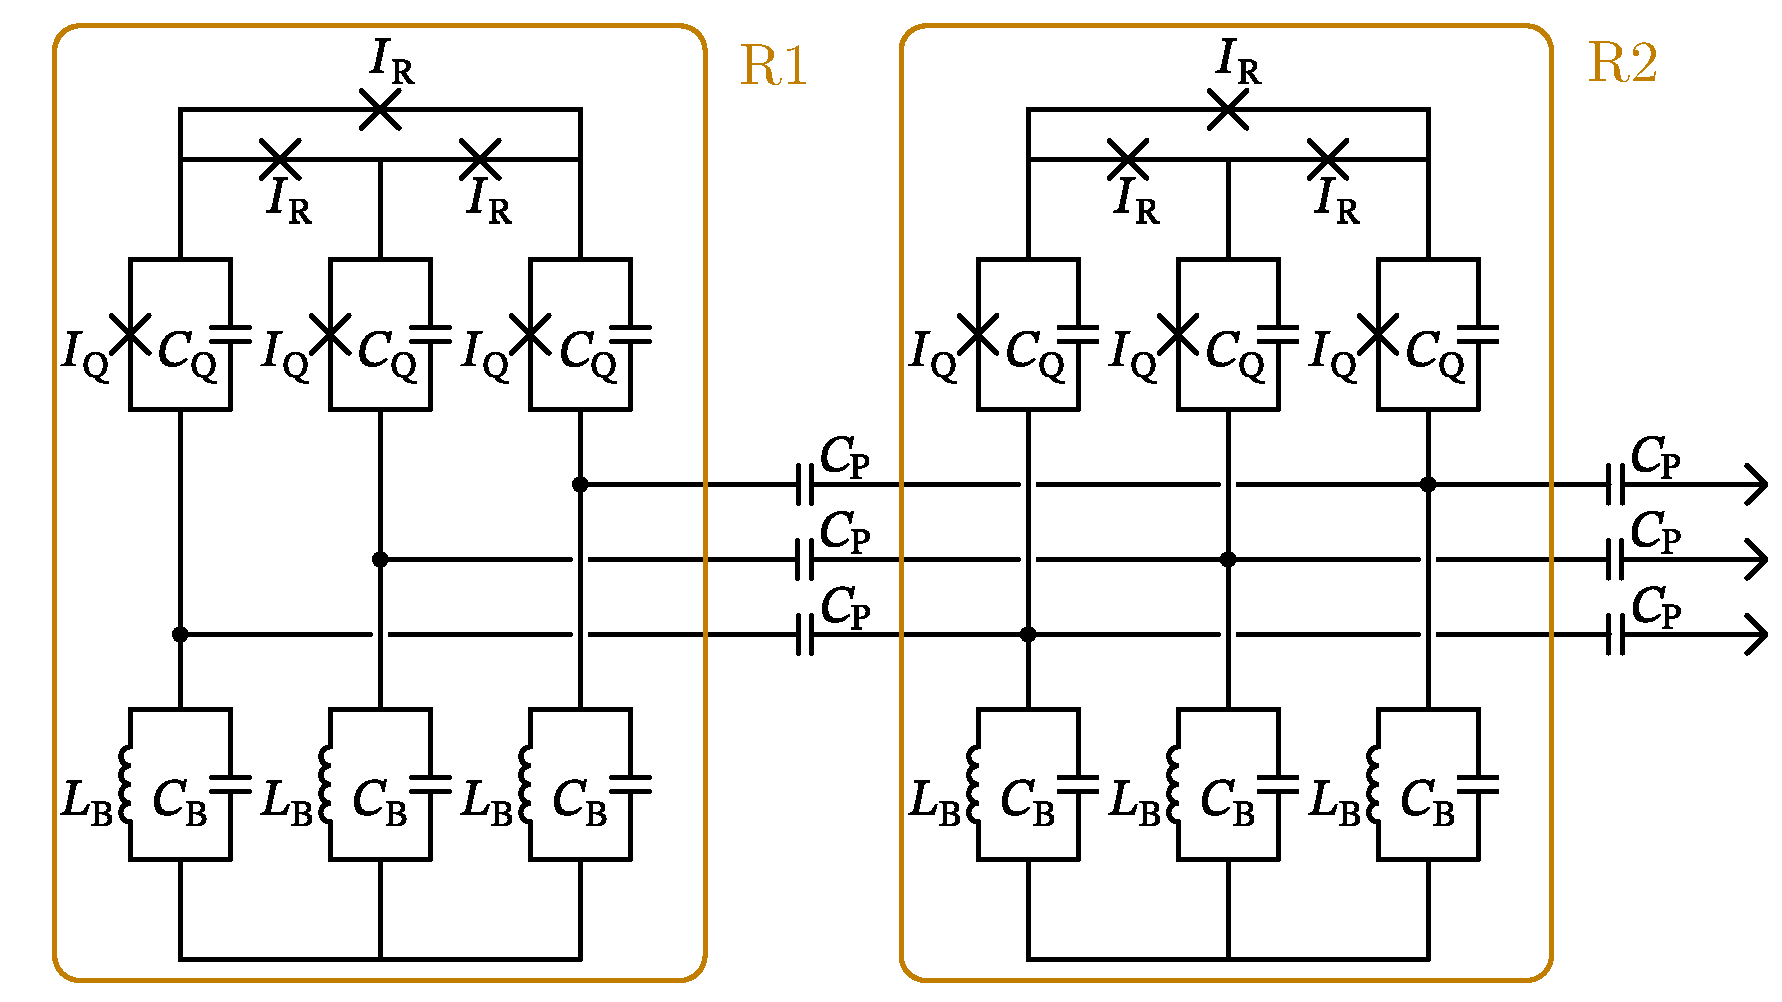
\includegraphics[width=\linewidth]{pics/SC_Potts_circuit_with_contours.pdf}
    \caption{Superconducting circuit implementation of the Potts model. It is composed from a chain of the $\Zthree$ Rabi model superconducting circuits $\mathrm{R1}$, $\mathrm{R2}$, etc [see Fig.~\ref{fig:superconducting-Rabi}]. The Potts model circuit is described by the Hamiltonian~\eqref{eq:coupled-rabi}. Subscript ``B'' denote elements corresponding to boson degrees of freedom; subscript ``Q'' denote qubit elements; subscript ``R'' denote elements responsible for interaction in qubit-boson ring; subscript ``P'' denote elements responsible for interaction in Potts model.}
    \label{fig:superconducting-potts}
\end{figure}

Having explored the theoretical construction of the Potts model based on a chain of the Rabi models, here we show how to implement the Potts model based on superconducting circuits. We consider a chain of the superconducting circuits simulating the $\Zthree$ Rabi models [see Sec.~\ref{sec:superconducting-implementation}]. Next, we need to couple the neighbor Rabi models with a boson hopping term to get the Hamiltonian~\eqref{eq:coupled-rabi}. As we have learned in Sec.~\ref{sec:underlying-qb-ring}, we have to couple the bosons modes of the neighbor QB rings pairwise to do it. Therefore, we connect the corresponding LC circuits of the neighbor QB rings by the inductive coupling (Fig.~\ref{fig:superconducting-potts}). Although capacitive coupling is more common, here it induces unwanted  all-to-all coupling. On the other hand, the inductive coupling leads us to the hopping term we want. First of all, the Hamiltonian terms corresponding to the inductors are:
\begin{equation}
\begin{aligned}
    &V_{\text{P},n,j} = \frac{1}{2L_{\text{P}}} (\hat \phi_{n+1,j} - \hat \phi_{n,j})^2 = \frac{\hat \phi_{n,j}^2 + \hat \phi_{n+1,j}^2}{2L_{\text{P}}} \\
    &- \frac{\hat b^{\dagger}_{n,j} \hat b^{\dagger}_{n+1,j} + \hat b^{\dagger}_{n,j} \hat b_{n+1,j} + \hat b_{n,j} \hat b^{\dagger}_{n+1,j} + \hat b_{n,j} \hat b_{n+1,j}}{4L_{\text{P}}C_{\text{B}}\Omega_{QB}} 
\end{aligned}
\end{equation}
where we expressed the flux operator through the creation and annihilation operators, $\hat \phi_{n,j} = (\hat b_{n,j} + \hat b_{n,j}^{\dagger})/\sqrt{2C_{\text{B}} \Omega_{QB}}$.

We ignore the $ \hat \phi_n^2 $ and $ \hat \phi_{n+1}^2 $ terms because they simply renormalize the Rabi model parameters. Additionally, the inductor coupling produces undesired terms $\hat b^{\dagger}_{n,j} \hat b^{\dagger}_{n+1,j}$ and $\hat b_{n,j} \hat b_{n+1,j}$. However, we can use the Rotating Wave Approximation (RWA) to eliminate them. For RWA to be applicable, we need $\Omega_{QB} = \sqrt{L_{\text{B}} C_{\text{B}}} \gg (L_{\text{P}} C_{\text{B}} \Omega_{\text{QB}})^{-1}$. After applying RWA, we are left precisely with the hopping term between the boson modes of the neighbor Rabi model. Consequently, in line with Sec.~\ref{sec:theoretical-potts} the superconducting circuit in Fig.~\ref{fig:superconducting-potts} models the $\Zthree$ Potts model. The coupling parameters of the resulting Potts model could be expressed through the circuit parameters:
\begin{equation}
\begin{aligned}
    &f_{\text{P}} = \frac{I_{\text{R}}}{2} \exp\left(-\frac{1}{2}\sqrt{\frac{L_{\text{B}}}{C_{\text{B}}}}\right), \\
    &J_{\text{P}} = \frac{1}{2L_{\text{P}}}\sqrt{\frac{L_{\text{B}}}{C_{\text{B}}}}. 
\end{aligned}
\end{equation}
\todo{Finishing remarks}

\subsection{Coupled optomechanical \texorpdfstring{$\Zthree$}{Z3} Rabi models}

\begin{figure}[t]
    \centering
    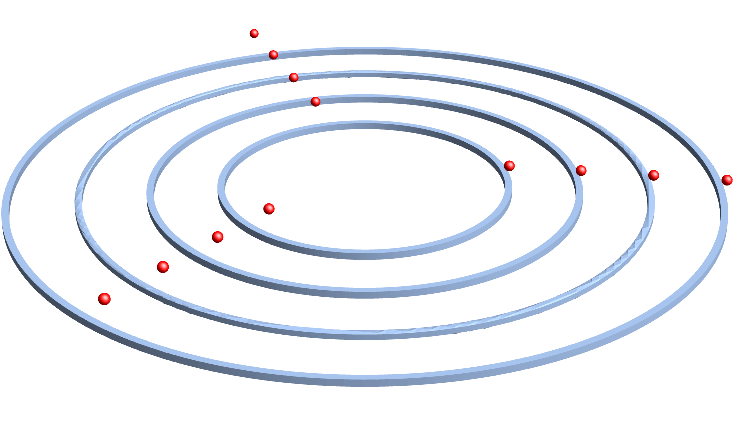
\includegraphics[width = 0.8 \linewidth]{pics/optomechanical_Potts_pic.pdf}
    \caption{Schematic illustration of the optomechanical (OM) implementation of the Potts model. It consists of several concentric OM implementations of the Rabi model, i.e., several concentric cyclic chiral waveguide and three trapped ions on top of each waveguide.}
    \label{fig:optomechanical-potts}
\end{figure}

We can repeat the same procedure for the optomechanical system. However, it is a bit more peculiar, because of the circular waveguide in the optomechanical Rabi model. To build the optomechanical $\Zthree$ Potts model we arrange the optomechanical $\Zthree$ Rabi model concentrically (see Fig. \ref{fig:optomechanical-potts}). On the one hand, the radius of the waveguide does not affect the parameters of the model, on the other hand, placing the ions of the neighbor Rabi models close to each other creates phonon-phonon interaction through the ion Coulomb interaction \cite{schneider_experimental_2012,timm_dynamics_2023}. The phonon-phonon interaction between the neighboring Rabi models leads to the Hamiltonian~\eqref{eq:coupled-rabi} and consequently to the $\Zthree$ Potts model as described before.


\subsection{Chiral Potts model and parafermions}


In this subsection, we want to briefly overview the chiral Potts model. It is a generalization of the ordinary Potts model that has a chiral nearest-neighbour interaction:
\begin{equation}
\label{eq:chiral-potts-hamiltonian}
\begin{aligned}
    H_{\text{chPotts}} = &f'\sum_{n=1}^L (e^{i\phi'} Z_n + e^{-i\phi'} Z_n^{\dagger}) \\
    &+ J' \sum (e^{i\theta'} X_n X_{n+1}^{\dagger} + e^{-i\theta'} X_n^{\dagger} X_{n+1}).
\end{aligned}
\end{equation}
In other words, it is simply the Potts model~\eqref{eq:potts-hamiltonian} with a complex parameter $J'$. 

In the construction described in Sec.~\ref{sec:potts-model}, the interaction parameter $J'$ originates from the neighbor QB ring boson interaction. Hence, if we want to engineer the chiral Potts model, we have to obtain a chiral boson-hopping term. To do it we need to break the time-reversal symmetry. It is difficult to do directly. However, if we consider a time-periodical coupling, then the effective interaction can be chiral \cite{roushan_chiral_2017, metelmann_nonreciprocal_2015, owens_quarterflux_2018}. A general way to obtain the chiral boson hopping was proposed in \cite{bermudez_synthetic_2011}. More specifically, the chiral boson hopping in the superconducting circuits can also be implemented \cite{}. \todo{Expand!}

\todo{Mention that the relation is the same as for the majoranas and Ising model} For the Potts model a generalization of the Jordan-Wigner transformation exists. It is called the Fradkin-Kadanoff (FK) transformation \cite{fradkin_disorder_1980}, and it allows us to rewrite $X_j, \, Z_j$ in terms of parafermions:
\begin{equation}
\Gamma_j = \prod\limits_{k<j} Z_k X_j , \quad \Delta_j = \prod\limits_{k\le j} Z_k X_j.
\end{equation}
Here $\Gamma_j, \, \Delta_j$ are parafermion operators with a parafermion commutation relation: $\Gamma_j \Gamma_k = \omega^{\sgn(j-k)} \Gamma_k \Gamma_j, \, \Delta_j \Delta_k = \omega^{\sgn(j-k)} \Delta_k \Delta_j$, and finally $\Gamma_j \Delta_k = \omega^{\sgn(j-k)} \Delta_k \Gamma_j$.

Using the FK transformation, it is easy to show that the Potts model is equivalent to a parafermion chain. The only problem is that FK transformation is not local. In terms of parafermion operators, the chiral Potts model Hamiltonian~\eqref{eq:chiral-potts-hamiltonian} looks like 
\begin{equation}
\begin{aligned}
    H_{\text{chPotts}} = &f' \sum \left( e^{i\phi'} \Gamma_j \Delta_j^{\dagger} + e^{-i\phi'} \Delta_j \Gamma_j^{\dagger}\right) \\
    &+J' \sum \left(e^{i\theta'} \Delta_j \Gamma_{j+1}^{\dagger} + e^{-i\theta'} \Gamma_{j+1} \Delta_j^{\dagger}\right).
\end{aligned}
\end{equation}

On the other hand, it is well-known that parafermion chain host a topological phase with the parafermion edge modes  \cite{fendley_parafermionic_2012}:
\begin{equation}
\Gamma_{\text{edge}} = \Gamma_1 + \frac{f'}{J' \sin(3\theta')} \mathcal{O} + \dots
\end{equation}

However, the parafermion edge mode is not localized after FK transformation. As a result, we do not have an actual topological phase in the chiral Potts model. However, having the exact mapping between the parafermion chain and the Potts model allows us to simulate the parafermion physics.



\section{Conclusion}
\label{sec:conclusion}

We introduced a hierarchy of $\Zthree$-symmetric systems. In the qubit-boson ring, the $\Zthree$ symmetry appears as a discrete rotational symmetry, whereas in the Rabi model, a specific sector of the qubit-boson ring, the symmetry acts as an internal one. This internal symmetry also exists in the $\Zthree$ Potts model, which we construct by coupling multiple $\Zthree$ Rabi models.

Our main goal was to suggest a way towards an experimental realization of the $\Zthree$ Rabi and Potts models. We believe that the proposed superconducting circuit is feasible. However, this approach does not have to be restricted only to the superconducting circuit platform. For example, we believe that a similar strategy work for the spin-qubit systems. Though, this remains a topic for a future research.

More broadly, our work highlights the intriguing potential of $\Zn$-symmetric systems within condensed matter physics. These systems present a fertile ground for discovering novel quantum phenomena, many of which are yet to be fully understood or described. We believe that the further investigation into these models reveals new insights and advance our understanding of symmetry in quantum systems.

\begin{comment}Our analysis yields three main results. (i) We derive the effective Hamiltonian for a $\Zthree$ Rabi system in which a cyclic three-level “artificial atom” couples to a cavity mode, guaranteeing microscopic $\Zthree$ charge conservation. (ii) We demonstrate a transition from a unique, symmetry-preserving ground state to a threefold-degenerate manifold, and identify the associated collective excitation—the “Potts mode”—that connects these ground states. (iii) Finite-size scaling confirms that the transition is genuinely second order. These findings establish a direct bridge between few-body light–matter models and Potts field theory and suggest that forthcoming superconducting-qutrit devices could probe $\Zthree$ criticality and its excitations in a controllable setting. The remainder of the paper presents the model, analytic framework, numerical results and experimental outlook in detail.
\end{comment}

\section*{Acknowledgments} 

We thank Daria Kalacheva, Henry Legg, Katharina Laubscher, and Ilia Luchnikov for fruitful discussions and useful comments. This work was supported as a part of NCCR SPIN, a National Centre of Competence in Research, funded by the Swiss National Science Foundation (grant number 225153). This work has received funding from the Swiss State Secretariat for Education, Research and Innovation (SERI) under contract number M822.00078.


\appendix

\section{Generalisation to an arbitrary interaction matrix}
\label{app:arbitrary-interaction-summary}

For completeness we summarise how the above derivation extends to a QB ring
with an arbitrary $\Zthree$--symmetric interaction matrix~$A$.  The starting
Hamiltonian is
\begin{equation}
\label{eq:arbitary-interaction-hamiltonian}
  \begin{aligned}
    \hat H_{\text{gen}} &= \epsilon \sum_{j=1}^{3} \sigma_j^z
      + \Omega \sum_{j=1}^{3} \hat a_j^{\dagger} \hat a_j + \hat V_{\text{gen}},
      \\
    \hat V_{\text{gen}} &= g \sum_{j,k} A_{jk}
      \sigma_j^{+} \sigma_k^{-} e^{ i ( \hat x_j - \hat x_k ) },
  \end{aligned}
\end{equation}
with $A^{\dagger}=A$.  The same sequence of steps---momentum translation $S$,
Fourier transform, and restriction to $\mathcal H_{\text{QB},1}$---again leads
to the two--mode Hamiltonian\footnote{An additional basis change might be
required to diagonalise the purely spin term.}
\eqref{eq:effective-rabi}, now with $gA$ replacing $g(Z+Z^{\dagger})$.  Hence any
interaction matrix compatible with $\Zthree$ symmetry can be mapped onto the
canonical Rabi model.  The parameter correspondence reads
\begin{equation}
  \Omega_R = \Omega, \qquad \lambda = \sqrt{ \frac{\Omega}{6 m} }.
\end{equation}

In the superconducting implementation one has $A = X + X^{\dagger}$, thereby
recovering the special case treated above.  The optomechanical realisation
gives rise to a different Hermitian $A$ but follows exactly the same logic.





\section{Charge qubit for the \texorpdfstring{$\Zthree$}{Z3} Rabi model}
\label{app:charge-qubit}


\begin{figure}[t]
    \centering
    \subfloat[]{
         \centering
         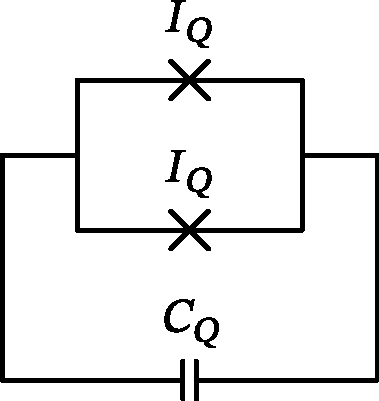
\includegraphics[width=0.4\linewidth]{pics/SC_qubit2_svg-tex.pdf}
         \vspace{0.1pt} %% Shifts the first image to allign it with x axis of the second image
         %%\caption{}
         \label{fig:2nd-harmonic-qubit-a}}
     \hfill
    \subfloat[]{
         \centering
         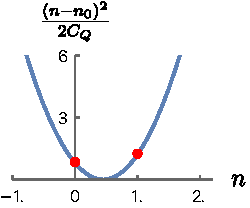
\includegraphics[width=0.5\linewidth]{pics/capacitor_potential.pdf}
         %%\caption{ }
         \label{fig:second-harmonic-qubit-b}}
    \caption{Second-harmonic qubit. a) The electric circuit of the second-harmonic qubit circuit. b) The capacitor potential~\eqref{eq:second-harmonic-qubit} for $n_0 = 0.45 = 0.5 - 0.05 $. The red dots show the eigenenergies of the second-harmonic qubit.}
    \label{fig:second-harmonic-qubit}
\end{figure}


The Cooper Pair Box (CPB) qubit is the most well-known type of charge qubit. However, it is not suitable for our purposes because its eigenstates are not charge states but their symmetric/antisymmetric combinations. Its Hamiltonian is proportional to $\sigma^x$. But in this case, the qubit chain Hamiltonian does not commute with total number of qubit excitations operator $S^z$.

Hence, we need another type of a charge qubit. Considering that the $\sigma^x$ term in the Hamiltonian arises from the JJ term the natural idea is to get rid of the JJ and consider a purely capacitor qubit. Although theoretically suitable for our purposes, without the JJ the charge qubit is very sensitive to noise. Therefore, it is not a realistic approach.

Consequently, we want two things simultaneously: Hamiltonian proportional to $\sigma^z$ in charge basis and JJ to fight noise. The solution turns out to be a higher harmonic Josephson junction. Usually it is neglected, but the JJ Hamiltonian always include higher harmonics as well
\begin{equation}
    \hat H_{JJ} = E_{J,1} \cos{\hat \phi} + E_{J,2} \cos{2\hat \phi} + \dots,
\end{equation}
where $\phi$ is the superconducting phase.

In practice, the higher harmonics are usually considerably weaker $E_{J,2} \ll E_{J,1}$. But if we were to eliminate the first harmonic completely, then we would be left with the second harmonic. The second harmonic, on the one hand, can help to supress the noise and, on the other hand, does not appear in the qubit Hamiltonian:
\begin{equation}
    \cos{2\hat \phi}\bigg|_{\mathcal{V}} = \frac{1}{2}\left(e^{2i\hat\phi} + e^{-2i\hat \phi}\right)\bigg|_{\mathcal{V}}=\frac{1}{2}\left((\sigma^+)^2 + (\sigma^-)^2\right) =0
\end{equation}

To eliminate the first harmonic, we can use a Superconducting Quantum Interference Device (SQUID) \cite{valentini_parityconserving_2024}. If the magnetic flux through the SQUID is tuned to $\Phi = \pi$, then the SQUID Hamiltonian looks like:
\begin{equation}
\begin{aligned}
    \hat H_{squid} = &I_{Q,1} \cos(\hat \phi) + I_{Q,2} \cos(2\hat \phi) + I_{Q,1} \cos(\hat \phi + \pi) \\
    &+ I_{Q,2} \cos(2\hat \phi + 2\pi) = 2 I_{Q,2} \cos(2\hat \phi).
\end{aligned}
\end{equation}
As a result, only the second harmonic is left.

Consequently, we can construct a qubit based on the second-harmonic JJ (see Fig. \ref{fig:second-harmonic-qubit}). It is described by the Hamiltonian:
\begin{equation}
\label{eq:second-harmonic-qubit}
    \hat H = \frac{1}{2C_Q} (\hat n - n_0)^2 + 2 I_{Q,2} \cos(2\hat\phi)
\end{equation}
If we tune $n_0$ a bit off 1/2: $n_0 = 0.5 - \delta$, then the qubit Hamiltonian looks like:
\begin{equation}
    \hat H_{\text{qubit}} = \frac{\delta}{2 C_Q} \sigma_z.
\end{equation}
Hence, we obtained the qubit Hamiltonian we wanted. Here we consider $\frac{1}{2C} \gg 2 E_{J,2}$ as usual for charge qubits.

To conclude, the charge qubit we have in mind consists of a capacitor and the second-harmonic JJ. One can think of it as a certain generalization of a Cooper Pair Box qubit. In this appendix, we only briefly described its blueprint to give additional substance to the proposal in Sec.~\ref{sec:superconducting-implementation}.


\section{Disorder in the superconducting implementation}
\label{app:disorder}
\subsection{Disorder breaking the total qubit excitation number conservation}


\begin{figure*}[th]
    \captionsetup[subfloat]{captionskip=-135pt} %%Moving captions on top
    \centering
    \subfloat[]{
         \centering
         %%\caption{}
        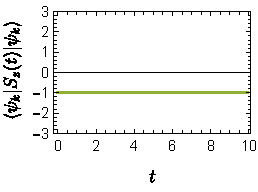
\includegraphics[width=0.32\linewidth]{pics/Spin_correlators_1.pdf}
         \label{fig:1st-spin-correlator}}
    \subfloat[]{
         \centering
        %%\caption{ }
        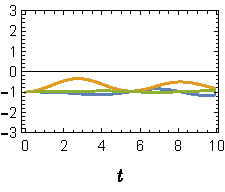
\includegraphics[width=0.274\linewidth]{pics/Spin_correlators_2.pdf}
         \label{fig:2nd-spin-correlator}}
    \subfloat[]{
         \centering
        %%\caption{}
        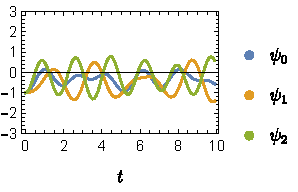
\includegraphics[width=0.37\linewidth]{pics/Spin_correlators_3.pdf}
         \label{fig:3rd-spin-correlator}}
    \caption{Time dependence of the total spin excitation operator. To illustrate robustness of the Rabi model implementation with the respect to the disorder~\eqref{eq:rabi-breaking-disorder} we plotted $\langle S_z(t) \rangle$. The standard variance of the disorder $\Delta_j$ equals for plot a) 0.1; b) 0.3; c) 1.}
    \label{fig:spin-excitation-plot}
\end{figure*}

First, while discussing the effect of the disorder on the qubit-boson ring~\eqref{eq:physical-hamiltonian}, we need to consider a term that breaks the conservation of the total excitation number of qubits $\hat S^z$. This conservation law is broken by the Zeeman terms being not perfectly aligned with $\hat z$ direction:
\begin{equation}
    \hat H_{QB,\text{dis}} = \hat H_{QB} + \sum_{j=1}^3 \Delta_j \sigma_j^x.
\end{equation}
As explained in App. \ref{app:charge-qubit}, $\Delta_j$ being equal to zero for qubit-boson ring based on superconducting circuits relies on the fine-tuning of the SQUID magnetic field. Therefore, in a realistic setting we unavoidably are going to have non-zero $\Delta_j = I_{Q,1}\sin(\Delta \Phi_j)$.



As a result, we have $[\hat H_{QB,\text{dis}}, \hat S^z] \neq 0 $. Unfortunately, it breaks the derivation of the Rabi model. However, assuming that the disorder is considerably smaller then other parameters in the Hamiltonian, we can still hope that the dynamics is approximately governed by the Rabi model. Because an analytic estimate is cumbersome, we performed numerical simulations of the qubit–boson ring. The results could be seen on Fig. \ref{fig:spin-excitation-plot}. The simulation shows that for the small disorder the qubit-boson ring stays around the single excitation subspace $\mathcal{H}_1$ because $\langle \hat S^z \rangle(t) \approx 1$. We speculate that it happens because the spins precess around $\langle \hat S^z \rangle = 1$.


\subsection{Disorder breaking \texorpdfstring{$\Zthree$}{Z3} symmetry}

\todo{Move the figure.}

Now, assuming that the total number of qubit excitations is conserved, we would like to investigate how the coordinate dependence of the parameter in the qubit-boson ring influences the resulting Rabi model. The spatial non-homogeneity obviously breaks the $\Zthree$ symmetry. However, we want to find the explicit symmetry-breaking term.
\begin{equation}
\label{eq:rabi-breaking-disorder}
\begin{aligned}
  \hat H_{QB}' &= \sum_j \epsilon_{j} \sigma_j^z + \sum_j \Omega_j \hat a^{\dagger}_j \hat a_j  \\
  &+ \sum_j g_{j,j+1} \left[\sigma_j^+ \sigma_{j+1}^- e^{i (\hat x_j - \hat x_{j+1})} +\text{h.c}\right]
\end{aligned}
\end{equation}
where we have
\begin{equation}
\begin{aligned}
    &\epsilon_j = \frac{\delta_j}{2 C_{Q,j}},\,
    \Omega_{QB,j} = \left(L_{\text{B},j}C_{\text{B},j}\right)^{-1/2}, \\
    &g_{j,j+1} = \frac{I_{\text{Rabi},j}}{2}.
\end{aligned}
\end{equation}

For brevity, we decompose the coupling parameters into a homogeneous part and a disorder: $\epsilon_j = \epsilon + \Delta \epsilon_j$, $\Omega_j = \Omega + \Delta \Omega_j$, $g_{j,j+1} = g + \Delta g_{j,j+1}$, where we assume that the disorder averaged over the coordinate is zero: $\sum_j \Delta \epsilon_j =  \sum_j \Delta \Omega_j = \sum_j \Delta g_{j,j+1} =0$. We can always achieve this by adjusting the homogeneous coupling.

Then the single-excitation sector is going to be described by
\begin{equation}
\begin{aligned}
    &\hat H_{\text{2 Rabi}}' = \hat H_{\text{2 Rabi}} + \epsilon(2) X \\
    &+\epsilon(1)  X^{\dagger} + (X + X^{\dagger}) \sum\limits_{k=1}^2 \Delta g(k) Z^k\\
    &+ \Omega(1) \sum\limits_{k=0}^2 \hat a^{\dagger}(k+1) \hat a(k) + \Omega(2) \sum\limits_{k=0}^2 \hat a^{\dagger}(k) \hat a(k+1) \\
    &+ \sum\limits_{l=1}^2 \frac{\Omega^{3/2}(l)}{2^{3/2}} \sum\limits_{k=0}^2 (\hat a(k+l) + \hat a^{\dagger}(-k-l)) Z^k.
\end{aligned}
\end{equation}

Due to the disorder the first boson mode does not decouple anymore. However, the structure of threefold cat state should be still conserved for small disorder. 



\bibliography{references}

\end{document}
